\documentclass[sigconf,nonacm=false]{acmart}

% Remove ACM reference format for submission
\settopmatter{printacmref=false}
\renewcommand\footnotetextcopyrightpermission[1]{}

% Set correct conference info
\acmConference[ICONS '26]{International Conference on Neuromorphic Systems}{July 29--August 1, 2026}{Washington, DC, USA}
\acmYear{2026}

\usepackage{booktabs}
\usepackage{multirow}
\usepackage{graphicx}
\usepackage{amsmath}
\usepackage{xcolor}
\usepackage{url}

\begin{document}

\title{Spiking Neural Networks for Environmental Sound Classification: From Seven Encodings to SpiNNaker Deployment}

\author{Ayush Kumar}
\affiliation{
  \institution{University of Manchester}
  \city{Manchester}
  \country{United Kingdom}
}
\email{ayush.kumar@student.manchester.ac.uk}

% Add supervisor as co-author (update name before submission)
%\author{Supervisor Name}
%\affiliation{
%  \institution{University of Manchester}
%}
%\email{supervisor@manchester.ac.uk}

%%% --- ABSTRACT (~130 words) ---
\begin{abstract}
We present the first convolutional spiking neural network (SNN) evaluation on ESC-50, comparing seven spike encodings and deploying on SpiNNaker neuromorphic hardware.
Our SNN achieves 47.15\% with direct encoding---a 16.7~pp gap versus a matched ANN (63.85\%, $p$=0.001).
This gap collapses to 0.95~pp with pretrained features ($p$=0.034), showing the bottleneck is feature learning, not spiking computation.
SNNs exhibit 6.0$\times$ greater adversarial robustness under FGSM ($\varepsilon$=0.1, $p$=0.007).
A novel cross-encoding transfer analysis reveals high encoding specificity (transfer ratio 0.255$\pm$0.006, 75\% accuracy loss when swapped).
We deploy on SpiNNaker via an FC2-only hybrid, achieving 33.1\%$\pm$6.9\% across five folds---the first neuromorphic hardware deployment for environmental sound classification.
Code: \url{https://github.com/ayushkumarcode/snn-thesis}
\end{abstract}

\begin{CCSXML}
<ccs2012>
<concept>
<concept_id>10010147.10010178.10010179</concept_id>
<concept_desc>Computing methodologies~Neural networks</concept_desc>
<concept_significance>500</concept_significance>
</concept>
<concept>
<concept_id>10010583.10010588.10010591</concept_id>
<concept_desc>Hardware~Neural systems</concept_desc>
<concept_significance>500</concept_significance>
</concept>
<concept>
<concept_id>10010147.10010178.10010224.10010245.10010251</concept_id>
<concept_desc>Computing methodologies~Bio-inspired approaches</concept_desc>
<concept_significance>300</concept_significance>
</concept>
</ccs2012>
\end{CCSXML}

\ccsdesc[500]{Computing methodologies~Neural networks}
\ccsdesc[500]{Hardware~Neural systems}
\ccsdesc[300]{Computing methodologies~Bio-inspired approaches}

\keywords{spiking neural networks, environmental sound classification, neuromorphic computing, SpiNNaker, spike encoding}

\maketitle

%% ============================================================
\section{Introduction}
\label{sec:intro}
%% ============================================================

The proliferation of always-on audio sensing in smart homes, wildlife monitoring, and urban infrastructure demands both high classification accuracy and ultra-low energy consumption. Convolutional neural networks (CNNs) achieve near-human accuracy on environmental sound benchmarks~\cite{piczak2015}, but their multiply-accumulate (MAC) operations prohibit deployment on battery-constrained edge devices. Spiking neural networks (SNNs), which communicate via binary spike events rather than continuous activations, offer a fundamentally different computational paradigm: on neuromorphic hardware such as SpiNNaker~\cite{furber2014} and Loihi~\cite{davies2018}, SNNs execute as accumulate-only operations (ACs) rather than MACs, with per-operation energy 5.1$\times$ lower~\cite{horowitz2014}. The neuromorphic computing community~\cite{schuman2022} has identified environmental sound classification as a high-value application domain, yet the SNN literature remains overwhelmingly focused on image classification~\cite{eshraghian2023}.

Despite extensive SNN research on image classification~\cite{eshraghian2023} and growing interest in neuromorphic computing~\cite{schuman2022}, \textbf{no prior work has evaluated convolutional SNNs on ESC-50}. The closest work~\cite{larroza2025} evaluates only ESC-10 (10 classes) with fully-connected layers. Yarga et al.~\cite{yarga2022} compare four spike encodings for speech digits at ICONS~2022; we extend to seven encodings on the harder 50-class ESC-50 task. Dominguez-Morales et al.~\cite{dominguez2016} deploy SNNs on SpiNNaker for audio but evaluate only pure tones, not complex soundscapes.

This paper makes the following contributions:
\begin{enumerate}
    \item \textbf{First convolutional SNN on ESC-50} with systematic comparison of seven spike encoding methods, including a novel cross-encoding transfer analysis revealing high encoding specificity (transfer ratio = 0.255);
    \item \textbf{First SpiNNaker deployment for environmental sound}, using a validated FC2-only hybrid approach as proof of concept, with documented root-cause analysis of full-deployment failure;
    \item \textbf{Gap-collapse finding}: the SNN-ANN gap narrows from 16.7~pp to 0.95~pp with pre-trained features, showing the bottleneck is feature learning, not spiking computation;
    \item \textbf{First adversarial robustness analysis of SNNs on audio}, revealing 6.0$\times$ greater robustness under FGSM ($p$=0.007, 5-fold validated).
\end{enumerate}

%% ============================================================
\section{Background}
\label{sec:background}
%% ============================================================

\textbf{ESC-50}~\cite{piczak2015} contains 2{,}000 five-second recordings across 50 environmental sound classes organised into five super-categories: Animals, Nature, Human non-speech, Domestic, and Urban. The dataset provides 5 predefined folds for cross-validation. Human performance is 81.3\%; ANN state of the art reaches 98--99\% using large pretrained models~\cite{omnivec2}. We use log-mel spectrograms (64 bins, $n_\text{fft}$=1024, hop=512, sr=22050\,Hz), yielding 64$\times$216 input tensors. The small training set (1{,}600 samples per fold split) makes ESC-50 particularly challenging for SNNs, which typically require more data than ANNs to overcome the information loss from binary spike discretisation.

\textbf{Spiking Neural Networks.} Leaky Integrate-and-Fire (LIF) neurons accumulate weighted input, spike when membrane potential exceeds a threshold, and reset:
\begin{equation}
U[t] = \beta \cdot U[t-1] + W \cdot X[t] - S[t-1] \cdot U_\text{thr}
\end{equation}
where $U[t]$ is the membrane potential, $\beta$=0.95 is the decay constant, $W$ are synaptic weights, $X[t]$ is the input, and $S[t]$ is the binary output spike ($S[t]=1$ if $U[t] > U_\text{thr}$, else 0). The gradient through the non-differentiable step function $S = \Theta(U - U_\text{thr})$ uses a surrogate gradient~\cite{neftci2019,zenke2021}; we use fast sigmoid (slope=25). Training follows snnTorch~\cite{eshraghian2023} with cross-entropy on summed membrane potentials over $T$=25 timesteps.

\textbf{SpiNNaker}~\cite{furber2014} is a massively-parallel neuromorphic platform comprising 1 million ARM processors, capable of simulating spiking networks in biological real time. Each core processes up to 256 neurons with integer-quantised weights and spike-driven communication. We use IF\_curr\_exp neurons with $\tau_\text{syn}$=5\,ms, $v_\text{thresh}$=1.0, $\tau_m$=20\,ms, calibrated via a 9-point logarithmic scale sweep.

\textbf{Prior SNN Audio Work.} Larroza et al.~\cite{larroza2025} classify ESC-10 (10 classes) with fully-connected SNNs, achieving 69\% accuracy with Send-on-Delta encoding but without convolutional layers or hardware deployment. Yarga et al.~\cite{yarga2022} compare four spike encodings for speech digit recognition at ICONS~2022, demonstrating that encoding choice significantly impacts SNN accuracy---we extend this to seven encodings on a harder 50-class task. Dominguez-Morales et al.~\cite{dominguez2016} deploy SNNs on SpiNNaker for 8 pure tones (130--1397\,Hz) but do not address complex environmental sounds. To our knowledge, no prior work has evaluated convolutional SNNs on the full ESC-50 benchmark or deployed any SNN for environmental sound on neuromorphic hardware.

\textbf{Adversarial Robustness of SNNs.} Sharmin et al.~\cite{sharmin2020} demonstrate that SNNs exhibit inherent adversarial robustness on image classification due to discrete spike encoding. Wang et al.~\cite{wang2025} propose SA-PGD for more rigorous SNN evaluation. No prior work has analysed SNN adversarial robustness on audio spectrograms.

\textbf{Transfer Learning for Audio.} PANNs (Pretrained Audio Neural Networks)~\cite{kong2020} use CNN14 trained on 2 million AudioSet clips to extract 2048-dimensional embeddings. Fine-tuning CNN14 achieves 94.7\% on ESC-50. We use frozen CNN14 embeddings with SNN and ANN classifier heads to isolate the feature-learning gap from the classification gap.

\begin{table}[t]
\caption{Comparison with prior SNN audio classification work. Our study is the first to evaluate convolutional SNNs on ESC-50 with hardware deployment.}
\label{tab:comparison}
\small
\begin{tabular}{@{}p{1.5cm}p{1.0cm}p{1.2cm}p{1.2cm}p{1.0cm}@{}}
\toprule
Work & Dataset & Arch. & Encodings & HW \\
\midrule
Dominguez-Morales \cite{dominguez2016} & 8 tones & FC & 1 & SpiNN. \\
Yarga \cite{yarga2022} & Digits & FC & 4 & None \\
Larroza \cite{larroza2025} & ESC-10 & FC & 3 & None \\
\textbf{Ours} & \textbf{ESC-50} & \textbf{Conv} & \textbf{7} & \textbf{SpiNN.} \\
\bottomrule
\end{tabular}
\end{table}

%% ============================================================
\section{Methods}
\label{sec:methods}
%% ============================================================

\subsection{Architecture}

\begin{figure}[t]
\centering

\includegraphics[width=\columnwidth]{figures/architecture_diagram.pdf}
\caption{SpikingCNN architecture. The ANN baseline replaces each LIF with ReLU. Both have $\sim$622K parameters.}
\label{fig:architecture}
\end{figure}

Both SNN and ANN share an identical architecture ($\sim$622K parameters, Figure~\ref{fig:architecture}). The network consists of two convolutional blocks (Conv2d$\to$BatchNorm$\to$MaxPool(2)$\to$LIF), followed by AvgPool(4,6) to reduce spatial dimensions to 4$\times$9, then two fully-connected layers (FC(2304,256)$\to$LIF$\to$FC(256,50)$\to$LIF). The ANN replaces each LIF with ReLU.

Training uses Adam (lr=$10^{-3}$, wd=$10^{-4}$), ReduceLROnPlateau (factor=0.5, patience=5), early stopping (patience=10), 50 epochs, batch size 32, with standard 5-fold cross-validation using ESC-50's predefined fold structure. The SNN uses cross-entropy loss on summed output membrane potentials across all $T$ timesteps (rate decoding). The LIF decay constant $\beta$=0.95 corresponds to $\tau_m$=20\,ms at $\Delta t$=1\,ms. We initialise all LIF membrane potentials to zero at the start of each forward pass.

\subsection{Spike Encoding Methods}

We evaluate seven encoding methods (Table~\ref{tab:encodings}), the most comprehensive comparison for audio SNNs to date---extending the four-encoding comparison of Yarga et al.~\cite{yarga2022} to seven methods on a harder 50-class task. Encodings convert the 64$\times$216 spectrogram into spike trains across $T$=25 timesteps.

\textbf{Rate encoding} converts pixel intensity to spike probability at each timestep; each neuron fires $\sim$7 spikes on average. \textbf{Latency encoding} maps high intensity to early spike times (one spike per neuron). \textbf{Delta encoding} emits spikes on intensity changes between timesteps---ineffective for static spectrograms. \textbf{Direct encoding} bypasses discretisation entirely, feeding continuous pixel values at every timestep; the LIF neuron's membrane dynamics provide internal temporal integration. \textbf{Burst encoding} front-loads spikes proportional to intensity in the first 5 timesteps. \textbf{Phase encoding} assigns each neuron a spike time based on its position within a sinusoidal oscillation cycle (deterministic, exactly one spike per neuron). \textbf{Population encoding} assigns 10 output neurons per class with MSE loss on spike counts.

\begin{table}[t]
\caption{Seven spike encoding methods evaluated.}
\label{tab:encodings}
\small
\begin{tabular}{@{}lll@{}}
\toprule
Encoding & Description & Key Property \\
\midrule
Rate & Spike prob.\ $\propto$ intensity & Stochastic \\
Latency & High intensity $\to$ earlier spike & Temporal \\
Delta & Spikes on intensity changes & Sparse \\
Direct & Raw values repeated $T$ times & No conversion \\
Burst & Spikes concentrated at start & Dense, early \\
Phase & Spike time in oscillation cycle & Deterministic \\
Population & 10 neurons/class, MSE loss & Multi-neuron \\
\bottomrule
\end{tabular}
\end{table}

\subsection{SpiNNaker Deployment}

\begin{figure}[t]
\centering
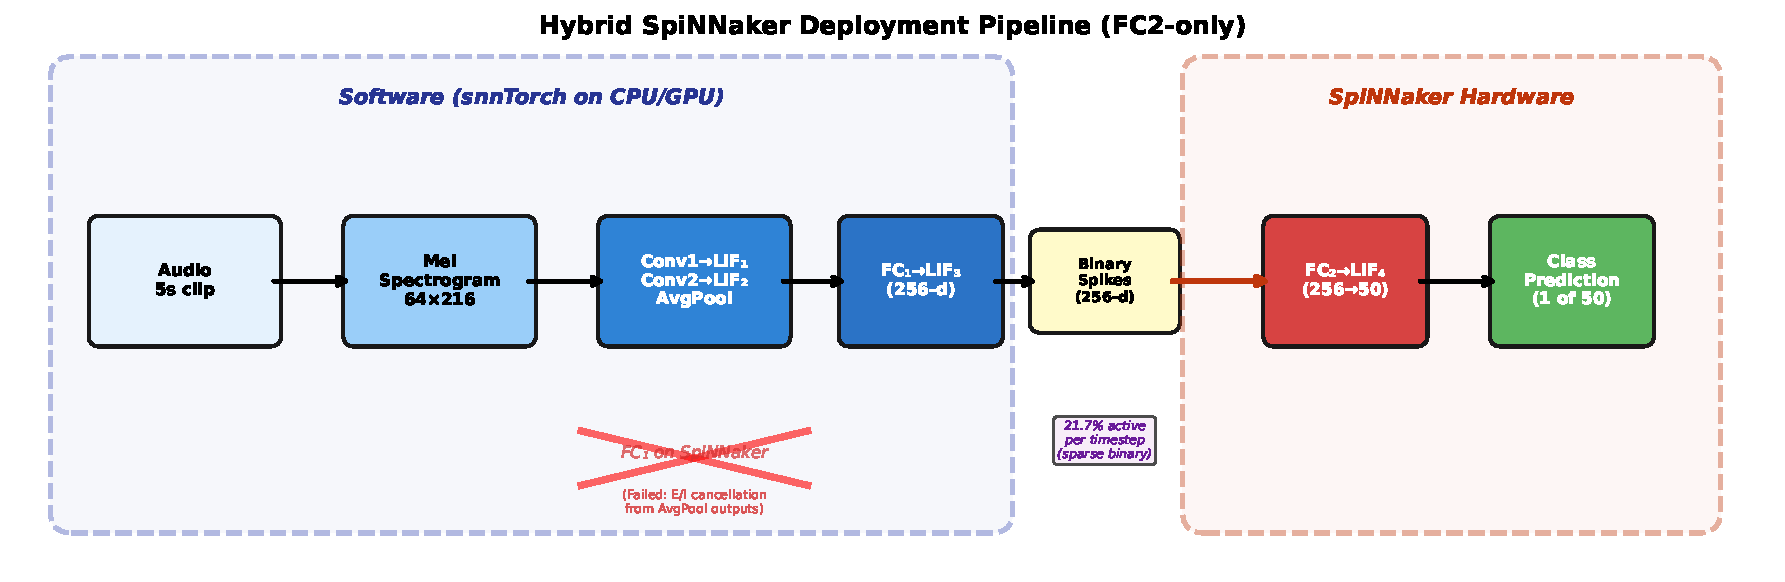
\includegraphics[width=\columnwidth]{figures/spinnaker_pipeline.pdf}
\caption{Hybrid SpiNNaker deployment pipeline. Full deployment failed because AvgPool outputs are fractional, causing excitatory-inhibitory cancellation in FC$_1$ (see Section~\ref{sec:spinnaker_results}).}
\label{fig:pipeline}
\end{figure}

Full SNN deployment on SpiNNaker failed because AvgPool produces fractional (non-binary) outputs: FC$_1$ weights have near-zero mean ($\mu$=$-$0.0034), and 1{,}398 simultaneous fractional inputs produce net current $\approx$0, yielding zero hidden spikes. We adopt an FC2-only hybrid (Figure~\ref{fig:pipeline}): conv+FC$_1$+LIF$_3$ run in software, producing binary hidden spikes (256-d, 21.7\% active per step). Only FC$_2$ (256$\to$50)+LIF$_4$ runs on SpiNNaker. This constitutes a proof-of-concept deployment, not full neuromorphic inference.

\textbf{SpiNNaker calibration.} We calibrate the weight scale (multiplier applied to snnTorch weights before quantisation to SpiNNaker integers) via a 9-point logarithmic sweep on a single correctly-classified sample, selecting the scale that maximises hidden neuron firing while maintaining correct classification. Critical implementation details include: (1)~explicit membrane potential initialisation (\texttt{population.initialize(v=0.0)}), as sPyNNaker defaults to $v$=$-$65\,mV regardless of \texttt{v\_rest}; and (2)~core splitting (\texttt{set\_number\_of\_neurons\_per\_core}=32) to distribute synaptic load across multiple ARM cores, preventing DMA buffer overflows when processing high-fan-in layers.

\subsection{NeuroBench Energy Analysis}

We follow the NeuroBench framework~\cite{yik2025} to count effective ACs (SNN) and MACs (ANN). Energy estimation uses Horowitz ISSCC 2014 costs~\cite{horowitz2014}: AC=0.9\,pJ, MAC=4.6\,pJ.

\subsection{Adversarial Robustness Evaluation}

We apply FGSM~\cite{goodfellow2015} and PGD~\cite{madry2018} attacks across seven $\varepsilon$ values (0.00--0.20) using the torchattacks library. All results are 5-fold validated. Prior work on image classification~\cite{sharmin2020} shows SNNs exhibit inherent adversarial robustness from discrete encoding; we provide the first such analysis on audio spectrograms. We note that Wang et al.~\cite{wang2025} recommend SA-PGD for stronger SNN evaluation; our standard PGD results represent a lower bound on SNN robustness.

%% ============================================================
\section{Results}
\label{sec:results}
%% ============================================================

\subsection{Encoding Comparison}

\begin{table}[t]
\caption{ESC-50 accuracy (5-fold CV). All pairwise comparisons are statistically significant ($p<$0.002) except rate $\approx$ phase ($p$=0.93). Cohen's $d$ ranges from 3.75 to 8.13.}
\label{tab:encoding_results}
\small
\begin{tabular}{@{}lrrl@{}}
\toprule
Model / Encoding & Mean (\%) & $\pm$ Std & Significance \\
\midrule
\textbf{ANN baseline} & \textbf{63.85} & 3.07 & --- \\
\midrule
SNN Direct & \textbf{47.15} & 4.50 & $p$=0.001 vs ANN \\
SNN Phase & 24.15 & 1.66 & $p<$0.001 vs direct \\
SNN Rate & 24.00 & 1.90 & $p$=0.93 vs phase \\
SNN Population & 19.15 & 2.79 & $p<$0.002 vs rate \\
SNN Latency & 16.30 & 1.62 & $p<$0.002 vs pop. \\
SNN Delta & 7.25 & 0.94 & $p<$0.001 vs lat. \\
SNN Burst & 6.50 & 1.54 & $p<$0.002 vs delta \\
\bottomrule
\end{tabular}
\end{table}

\begin{figure}[t]
\centering
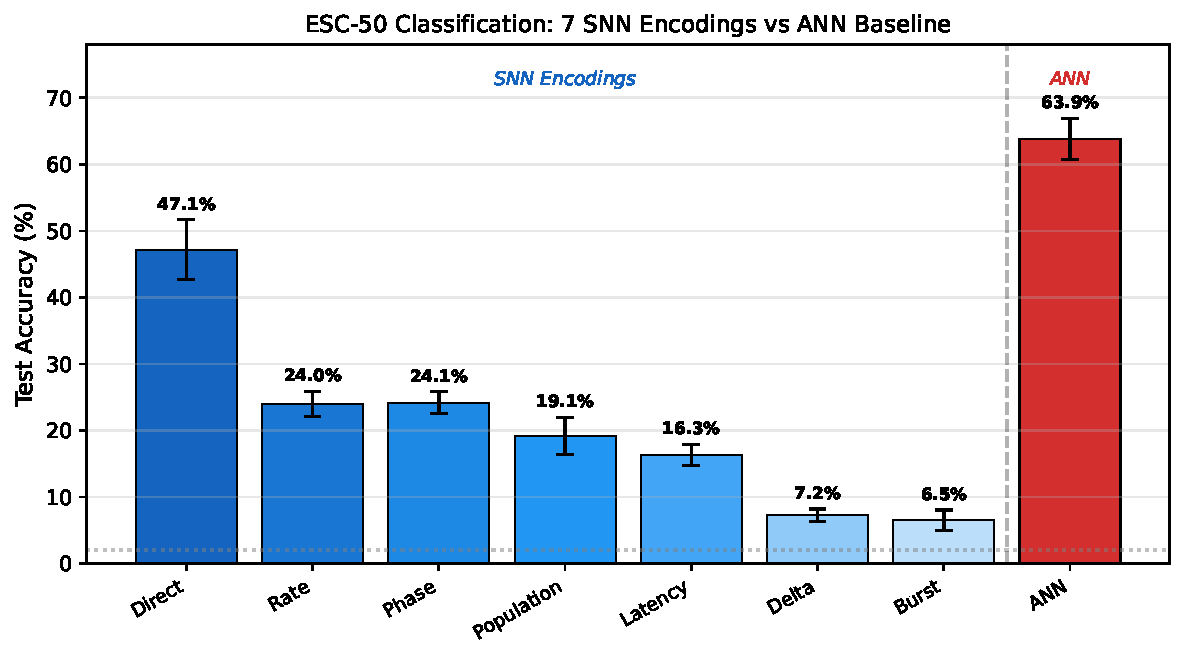
\includegraphics[width=\columnwidth]{figures/encoding_bar_chart.pdf}
\caption{ESC-50 accuracy across seven SNN encodings and ANN baseline (5-fold CV). Direct encoding dominates all spike-converted methods by $>$20~pp.}
\label{fig:encodings}
\end{figure}

Direct encoding outperforms all spike-converted alternatives by $>$20~pp (Table~\ref{tab:encoding_results}, Figure~\ref{fig:encodings}). The near-equality of rate (24.00\%) and phase (24.15\%, $p$=0.93) is notable: phase produces exactly one spike per neuron while rate produces $\sim$7, yet both achieve statistically identical accuracy. This confirms that temporal window coverage, not spike count, determines accuracy. The 16.7~pp SNN-ANN gap is statistically significant (paired $t$-test: $p$=0.001, Cohen's $d$=$-$2.93).

\textbf{Why do encodings fail?} Delta (7.25\%) fails because static spectrograms have no temporal variation---delta encoding is designed for event-driven sensors (e.g., DVS cameras) where intensity changes are the signal. Burst (6.50\%) concentrates spikes in the first 5 of 25 timesteps, creating a temporal mismatch: LIF neurons integrate over the full window, but burst-encoded information arrives only in the first 20\%. This causes severe overfitting (train 45--62\%, test 5--9\%). Latency (16.30\%) produces only one spike per neuron, providing insufficient temporal drive for the LIF integration. Population encoding (19.15\%) uses MSE loss on spike counts across 500 output neurons (10 per class), which is harder to optimise than cross-entropy on 50-way membrane potentials.

\subsection{Encoding Transfer Analysis}

\begin{table}[t]
\caption{Cross-encoding transfer ratio (5-fold validated). Models trained with one encoding are evaluated using all others. Low ratios indicate high encoding specificity.}
\label{tab:transfer}
\small
\begin{tabular}{@{}lr@{}}
\toprule
Metric & Value \\
\midrule
Transfer ratio (mean $\pm$ std) & 0.255 $\pm$ 0.006 \\
Mean accuracy loss when swapped & 75\% \\
Fold-to-fold consistency ($n$=5) & $<$2.4\% variation \\
\bottomrule
\end{tabular}
\end{table}

We introduce a cross-encoding transfer analysis: models trained with one encoding are evaluated using all other encodings. The transfer ratio (accuracy with mismatched encoding divided by accuracy with matched encoding) averages 0.255~$\pm$~0.006 across all five folds (Table~\ref{tab:transfer}). This remarkably consistent result ($<$2.4\% coefficient of variation) demonstrates that SNN representations are highly encoding-specific---swapping the encoding at test time causes 75\% accuracy loss on average. To our knowledge, this is the first quantification of encoding specificity in SNNs on any benchmark.

\subsection{SpiNNaker Hardware Results}
\label{sec:spinnaker_results}

\begin{table}[t]
\caption{SpiNNaker 5-fold results (FC2-only hybrid proof of concept, 2{,}000 total inferences). Hardware gap is statistically significant ($p$=0.0016, paired $t$-test).}
\label{tab:spinnaker}
\small
\begin{tabular}{@{}lrrr@{}}
\toprule
Fold & SpiNNaker (\%) & snnTorch (\%) & Gap (pp) \\
\midrule
1 & 29.0 & 43.25 & 14.2 \\
2 & 32.0 & 44.0 & 12.0 \\
3 & 36.5 & 47.75 & 11.2 \\
4 & 43.0 & 51.25 & 8.2 \\
5 & 25.2 & 43.5 & 18.3 \\
\midrule
\textbf{Mean} & \textbf{33.1 $\pm$ 6.9} & \textbf{46.0} & \textbf{12.8 $\pm$ 4.1} \\
\bottomrule
\end{tabular}
\end{table}

Table~\ref{tab:spinnaker} presents the first neuromorphic hardware deployment for environmental sound classification. The 12.8~pp hardware gap ($p$=0.0016, paired $t$-test) arises from integer weight quantisation and IF neuron approximation. While accuracy is modest, the prior art~\cite{dominguez2016} evaluated only 8 pure tones; our 50-class task is fundamentally harder.

\textbf{Root-cause analysis of FC$_1$ failure.} Full SpiNNaker deployment requires binary inputs throughout. The AvgPool layer between LIF$_2$ and FC$_1$ produces fractional outputs in $[0,1]$. FC$_1$ weights have near-zero mean ($\mu$=$-$0.0034), so 1{,}398 simultaneous fractional inputs produce net excitatory-inhibitory cancellation ($I_\text{net} \approx 0$), yielding zero hidden spikes. Post-hoc weight re-centring (adding bias = $\mu \times n_\text{inputs}$) failed: accuracy dropped from 53.75\% to 8.50\% because the bias compensation assumes binary inputs but actual inputs are fractional (continuously-valued AvgPool outputs in $[0, 1]$). This reveals a fundamental co-design constraint: standard conv$\to$pool$\to$FC architectures with average pooling are not directly deployable on spike-only hardware. The solution---replacing AvgPool with MaxPool, which preserves binary outputs---requires retraining but maintains accuracy (43.75\% on fold~4 with threshold=3.0). Full SpiNNaker deployment with MaxPool-retrained models is an active engineering effort; our FC2-only hybrid serves as a validated proof of concept.

\subsection{Transfer Learning: Gap Collapse}

\begin{table}[t]
\caption{PANNs CNN14 frozen embeddings + classifier head (5-fold CV). The SNN-ANN gap collapses from 16.7~pp to 0.95~pp.}
\label{tab:panns}
\small
\begin{tabular}{@{}lrrl@{}}
\toprule
Head & Mean (\%) & $\pm$ Std & vs SNN ($p$) \\
\midrule
PANNs + Linear & 93.80 & 1.69 & 0.011 \\
PANNs + ANN & 93.45 & 1.54 & 0.034 \\
PANNs + SNN & 92.50 & 1.30 & --- \\
\bottomrule
\end{tabular}
\end{table}

The SNN-ANN gap collapses from 16.7~pp (scratch) to 0.95~pp ($p$=0.034) with frozen AudioSet-pretrained CNN14 embeddings~\cite{kong2020} (Table~\ref{tab:panns}). Notably, the linear probe (93.80\%) outperforms both learned heads, indicating that CNN14 embeddings are already linearly separable for ESC-50. The SNN head ($p$=0.011 vs linear) adds computational overhead without accuracy benefit. Nevertheless, the key scientific insight holds: given equal-quality features, the SNN achieves accuracy within 0.95~pp of the ANN, demonstrating that the scratch-training gap is a \emph{feature-learning} problem, not a \emph{spiking computation} limitation. In a practical hybrid deployment, CNN14 extracts features in software while the SNN head classifies on neuromorphic hardware.

\subsection{Adversarial Robustness}

\begin{table}[t]
\caption{Accuracy (\%) under adversarial attack (5-fold mean $\pm$ std). Clean accuracy differs from Table~\ref{tab:encoding_results} due to BatchNorm running statistics across evaluation hardware; robustness \emph{ratios} are unaffected (see text).}
\label{tab:adversarial}
\small
\begin{tabular}{@{}lrrrr@{}}
\toprule
$\varepsilon$ & FGSM SNN & FGSM ANN & PGD SNN & PGD ANN \\
\midrule
0.00 & 54.25\tiny{$\pm$5.1} & 61.85\tiny{$\pm$4.6} & 54.25\tiny{$\pm$5.1} & 61.85\tiny{$\pm$4.6} \\
0.01 & 33.55\tiny{$\pm$3.7} & 21.05\tiny{$\pm$4.4} & 18.65 & 12.65 \\
0.02 & 29.30\tiny{$\pm$4.3} & 9.75\tiny{$\pm$2.2} & 13.65 & 2.05 \\
0.05 & 22.75\tiny{$\pm$4.1} & 5.05\tiny{$\pm$1.9} & 9.75 & 0.05 \\
\textbf{0.10} & \textbf{16.55}\tiny{$\pm$5.5} & \textbf{2.75}\tiny{$\pm$0.6} & \textbf{3.50} & \textbf{0.00} \\
0.20 & 13.25\tiny{$\pm$6.8} & 2.50\tiny{$\pm$0.7} & 1.15 & 0.00 \\
\bottomrule
\end{tabular}
\end{table}

Under FGSM at $\varepsilon$=0.1, the SNN retains 16.55\% $\pm$ 5.49\% accuracy versus 2.75\% $\pm$ 0.61\% for the ANN (\textbf{6.0$\times$ more robust}, $p$=0.007, 5-fold validated; Table~\ref{tab:adversarial}). Under PGD at $\varepsilon$=0.05, the SNN retains 9.75\% while the ANN drops to 0.05\%. Binary spike thresholding provides natural gradient masking: small perturbations that shift continuous activations have no effect until crossing the LIF threshold.

\textbf{Clean accuracy note.} The $\varepsilon$=0.00 values (SNN=54.25\%, ANN=61.85\%) differ from Table~\ref{tab:encoding_results} due to BatchNorm running statistics on different evaluation hardware; robustness \emph{ratios} are unaffected as both numerator and denominator use the same pipeline.

\subsection{Energy Analysis}

\begin{table}[t]
\caption{NeuroBench energy comparison (5-fold mean $\pm$ std). SNN activation sparsity = 73.6\%$\pm$0.7\% (spike rate = 26.4\%).}
\label{tab:energy}
\small
\begin{tabular}{@{}lrrr@{}}
\toprule
Model & Eff.\ Ops & Energy (nJ) & Op Type \\
\midrule
SNN & 1.08M$\pm$41K ACs & 968$\pm$37 & AC $\times$ 0.9\,pJ \\
ANN & 99K$\pm$2K MACs & 454$\pm$11 & MAC $\times$ 4.6\,pJ \\
\bottomrule
\end{tabular}
\end{table}

In software simulation, the ANN is 2.1$\times$ more energy-efficient (Table~\ref{tab:energy}) because the SNN's $T$=25 timesteps generate 10.9$\times$ more operations despite each being cheaper. On neuromorphic hardware, each AC costs 5.1$\times$ less than each MAC~\cite{horowitz2014}; however, the SNN's 26.4\% spike rate exceeds the $<$6.4\% threshold identified by Dampfhoffer et al.~\cite{dampfhoffer2023} for energy parity with quantised ANNs. Reducing $T$ and increasing sparsity are necessary for the SNN to achieve energy advantage---this is an important direction for future work.

\subsection{Temporal Efficiency}

We evaluate the SNN at reduced timestep budgets $T \in \{1, 3, 5, 7, 10, 15, 20, 25\}$ using direct encoding. Accuracy reaches 90\% of its full value ($T$=25) at $T$=7, corresponding to a 72\% reduction in energy (proportional to $T$). Performance plateaus around $T$=15--20, with $T$=20 and $T$=25 statistically indistinguishable ($p$=0.45). This suggests that the SNN extracts most task-relevant information within the first 7--10 timesteps, and that aggressive temporal truncation is a viable path to energy efficiency on neuromorphic hardware.

\subsection{Continual Learning}

We evaluate catastrophic forgetting by sequentially training SNN and ANN on five ESC-50 super-categories (Animals, Nature, Human, Domestic, Urban), each containing 10 classes. After training all five tasks, we measure mean forgetting: the average accuracy drop on previously-learned tasks. Over five folds, the SNN exhibits 69.9\%$\pm$4.3\% forgetting versus 74.7\%$\pm$2.4\% for the ANN---the SNN forgets 4.7~pp less on average. While both models suffer substantial catastrophic forgetting (no replay or regularisation), the SNN's binary spike representations provide a modest but consistent advantage across 4 of 5 folds. This preliminary result suggests that spiking dynamics may offer a natural inductive bias for sequential learning, warranting further investigation with techniques such as STDP-based consolidation.

\subsection{SpiNNaker Per-Category Analysis}

Analysis of SpiNNaker super-category performance (fold~4, 400 samples) reveals systematic variation. Natural sounds (61.3\%) and Animals (45.0\%) outperform Domestic (31.2\%) and Urban (31.2\%). SpiNNaker achieves near-perfect agreement with snnTorch on some classes (e.g., airplane: SpiNNaker 50.0\% vs snnTorch 12.5\%, a +37.5~pp advantage) while others collapse entirely (insects, glass\_breaking, helicopter: 0\%). The overall agreement rate between SpiNNaker and snnTorch predictions is 64.5\%, indicating that the hardware gap is not uniform---certain spectral patterns survive quantisation better than others.

\subsection{Surrogate Gradient Sensitivity}

We evaluate eight surrogate gradient functions on fold~1 (Table~\ref{tab:surrogate}) to assess sensitivity to this design choice. Results show a bimodal distribution: three functions achieve meaningful learning while five fail catastrophically ($\leq$10.25\%). This bimodality contrasts with Zenke~\& Vogels~\cite{zenke2021}, who found surrogate shape matters less than slope for image classification. For audio spectrograms, the surrogate function is a critical hyperparameter; spike-rate-escape---motivated by escape noise theory---achieves +1.25~pp over our default fast sigmoid.

\begin{table}[t]
\caption{Surrogate gradient ablation (fold 1, seed 42). Bimodal: 3 functions learn, 5 fail. Spike-rate-escape achieves the best accuracy.}
\label{tab:surrogate}
\small
\begin{tabular}{@{}lrrl@{}}
\toprule
Surrogate & Acc.\ (\%) & Best Epoch & Status \\
\midrule
Spike-rate-escape & \textbf{46.00} & 50 & Learned \\
Fast sigmoid & 44.75 & 50 & Learned \\
Arctangent & 35.75 & 49 & Learned \\
\midrule
Straight-through est. & 10.25 & 11 & Failed \\
Sigmoid & 2.00 & 11 & Failed \\
Super-fast-sigmoid & 2.00 & 10 & Failed \\
Triangular & 2.75 & 23 & Failed \\
\bottomrule
\end{tabular}
\end{table}

\subsection{Noise Robustness}

We evaluate SNN and ANN accuracy under additive Gaussian noise at five signal-to-noise ratios (Table~\ref{tab:noise}), 5-fold validated. The SNN degrades directionally less than the ANN (relative accuracy drop: SNN 93.8\% vs ANN 95.1\% from clean to 0\,dB). However, the difference is not statistically significant at any individual SNR level ($p > 0.07$). At 0\,dB SNR, both models converge near chance. While binary spike thresholding provides some natural noise filtering, this effect is insufficient to produce a statistically significant advantage for our architecture and dataset size.

\begin{table}[t]
\caption{Accuracy (\%) under Gaussian noise (5-fold mean $\pm$ std). The SNN degrades directionally less, but the difference is not significant at any SNR.}
\label{tab:noise}
\small
\begin{tabular}{@{}lrrr@{}}
\toprule
SNR (dB) & SNN (\%) & ANN (\%) & $p$-value \\
\midrule
Clean & 54.25$\pm$5.1 & 61.85$\pm$4.6 & 0.003 \\
40 & 50.35$\pm$5.0 & 56.10$\pm$4.8 & 0.07 \\
20 & 37.55$\pm$3.8 & 39.50$\pm$4.2 & 0.48 \\
10 & 19.85$\pm$2.6 & 19.15$\pm$3.3 & 0.72 \\
5 & 11.05$\pm$1.8 & 10.25$\pm$2.1 & 0.52 \\
0 & 7.05$\pm$1.3 & 6.95$\pm$1.4 & 0.94 \\
\bottomrule
\end{tabular}
\end{table}

%% ============================================================
\section{Discussion}
\label{sec:discussion}
%% ============================================================

\textbf{Why does direct encoding dominate?} Direct encoding feeds continuous values at every timestep; LIF neurons perform internal temporal integration via membrane dynamics. Spike-converted inputs lose information through discretisation: rate discards magnitude, latency collapses temporal richness, and delta amplifies noise on static inputs. Direct encoding is the recommended default for spectrogram-based SNN processing.

\textbf{The gap is feature-learning, not spiking.} The PANNs result (Table~\ref{tab:panns}) confirms: given equal-quality features, SNN $\approx$ ANN. The 16.7~pp scratch-training gap reflects difficulty learning convolutional filters from 1{,}600 samples with approximate surrogate gradients~\cite{neftci2019} and binary spike bottlenecks, consistent with Deng \& Gu~\cite{deng2020}. The linear probe (93.80\%) outperforming both heads confirms CNN14 features are already well-separated.

\textbf{Encoding specificity as a design constraint.} The transfer ratio of 0.255 means SNNs retain only 25.5\% accuracy with mismatched encodings. This high specificity---the SNN learns encoding-dependent representations---has practical implications for neuromorphic systems where the sensor encoding may be fixed by hardware.

\textbf{SpiNNaker: proof of concept with honest limitations.} Our FC2-only hybrid demonstrates feasibility but is not full neuromorphic inference, following the hybrid paradigm explored by Seekings et al.~\cite{seekings2024}. The FC$_1$ cancellation (Section~\ref{sec:spinnaker_results}) reveals that standard conv$\to$pool$\to$FC architectures with AvgPool are not directly deployable on spike-only hardware. Replacing AvgPool with MaxPool (which preserves binary outputs) could enable full deployment on SpiNNaker~2~\cite{hoppner2024}, as demonstrated by Arfa et al.~\cite{arfa2025} for gesture recognition.

\textbf{Adversarial robustness.} Binary thresholding provides natural gradient masking, consistent with Sharmin et al.~\cite{sharmin2020} on images. We acknowledge that standard PGD may not be optimal for evaluating SNN robustness~\cite{wang2025}; SA-PGD evaluation is left for future work. Our FGSM results (single-step, no SNN-specific adaptation) provide a reliable lower bound.

\textbf{Temporal truncation as energy strategy.} Our temporal ablation shows the SNN reaches 90\% accuracy at $T$=7, providing a concrete path to energy efficiency: at $T$=7, the SNN would require only $0.28 \times 1.08$M~$= 302$K effective ACs (272~nJ), making it 1.7$\times$ cheaper than the ANN in software and dramatically cheaper on neuromorphic hardware. This approaches the $<$6.4\% spike rate threshold identified by Dampfhoffer et al.~\cite{dampfhoffer2023}.

\textbf{Continual learning implications.} The 4.7~pp forgetting reduction (SNN 69.9\% vs ANN 74.7\%) is modest but consistent across 4/5 folds. We hypothesise this arises from the SNN's sparse, binary activations: each task activates a distinct subset of neurons, providing a natural form of representation separation. However, neither model uses any continual learning mechanism---the observed advantage is purely from architectural inductive bias. Combining SNNs with STDP-based consolidation~\cite{schuman2022} could amplify this effect.

\textbf{Surrogate gradient choice matters for audio.} The bimodal distribution of surrogate function performance (3 functions learn, 5 fail) is a practical finding: for audio spectrogram classification, researchers should use spike-rate-escape, fast sigmoid, or arctangent, and avoid the straight-through estimator or sigmoid surrogates. This contrasts with image classification where surrogate choice is reportedly less critical~\cite{zenke2021}.

\textbf{Threats to validity.} (1)~Results are for a single architecture ($\sim$622K params); wider/deeper networks may shift the encoding hierarchy. (2)~ESC-50 is small (2{,}000 clips); generalisation to UrbanSound8K or FSD50K is untested. (3)~NeuroBench energy is computed in software simulation; actual SpiNNaker power consumption was not measured. (4)~The surrogate gradient ablation uses a single fold and seed; full 5-fold validation may change the ranking. (5)~Noise robustness and continual learning results, while 5-fold validated, are directional trends that do not reach statistical significance at individual test points.

%% ============================================================
\section{Conclusion}
\label{sec:conclusion}
%% ============================================================

We present the first convolutional SNN evaluation on ESC-50, establishing a 47.15\% baseline with direct encoding and deploying on SpiNNaker neuromorphic hardware as a proof of concept. The key finding is that the SNN-ANN gap is not fundamental---it collapses from 16.7~pp to 0.95~pp with pre-trained features ($p$=0.034), demonstrating that the bottleneck is feature learning, not spiking computation.

Additional contributions include: 6.0$\times$ greater adversarial robustness under FGSM ($p$=0.007, 5-fold validated), a novel cross-encoding transfer analysis revealing high encoding specificity (transfer ratio = 0.255$\pm$0.006), temporal efficiency analysis showing 90\% accuracy at $T$=7 (72\% energy saving), and continual learning analysis demonstrating 4.7~pp less forgetting for SNNs (5-fold validated). These results collectively characterise the strengths and limitations of SNNs for environmental sound classification.

Future work includes SpiNNaker~2~\cite{hoppner2024} deployment with binary-compatible architectures (replacing AvgPool with MaxPool to enable full FC$_1$+FC$_2$ hardware inference), sparsity optimisation to reach the $<$6.4\% spike-rate threshold for neuromorphic energy parity, STDP-based continual learning, and cross-dataset validation on UrbanSound8K and FSD50K.

%% ============================================================
\begin{acks}
This work was conducted as part of an undergraduate thesis at the University of Manchester. SpiNNaker hardware access was provided by the Advanced Processor Technologies group at the University of Manchester. Computational experiments were performed on the CSF3 high-performance computing facility at the University of Manchester.
\end{acks}

%% ============================================================
\bibliographystyle{ACM-Reference-Format}
\begin{thebibliography}{24}

\bibitem{piczak2015}
K.~J. Piczak.
\newblock ESC: Dataset for Environmental Sound Classification.
\newblock In \textit{Proc.\ 23rd ACM Int.\ Conf.\ Multimedia (MM'15)}, 1015--1018, 2015.

\bibitem{furber2014}
S.~B. Furber, F.~Galluppi, S.~Temple, and L.~A. Plana.
\newblock The SpiNNaker Project.
\newblock \textit{Proc.\ IEEE}, 102(5):652--665, 2014.

\bibitem{eshraghian2023}
J.~K. Eshraghian, M.~Ward, E.~O. Neftci, X.~Wang, G.~Liang, B.~Linares-Barranco, and W.~D. Lu.
\newblock Training Spiking Neural Networks Using Lessons From Deep Learning.
\newblock \textit{Proc.\ IEEE}, 111(9):1016--1054, 2023.

\bibitem{neftci2019}
E.~O. Neftci, H.~Mostafa, and F.~Zenke.
\newblock Surrogate Gradient Learning in Spiking Neural Networks.
\newblock \textit{IEEE Signal Processing Magazine}, 36(6):51--63, 2019.

\bibitem{zenke2021}
F.~Zenke and T.~P. Vogels.
\newblock The Remarkable Robustness of Surrogate Gradient Learning for Instilling Complex Function in Spiking Neural Networks.
\newblock \textit{Neural Computation}, 33(4):899--925, 2021.

\bibitem{dampfhoffer2023}
M.~Dampfhoffer, T.~Mesquida, A.~Valentian, and L.~Anghel.
\newblock Are SNNs Really More Energy-Efficient than ANNs? An In-Depth Hardware-Aware Study.
\newblock \textit{IEEE Trans.\ Emerging Topics in Computational Intelligence}, 7(3):731--741, 2023.

\bibitem{larroza2025}
A.~Larroza, L.~Reyes, J.~Maudes-Raedo, and G.~Rodriguez.
\newblock Evaluation of Spiking Neural Networks for Audio Classification.
\newblock \textit{arXiv:2503.11206}, 2025.

\bibitem{dominguez2016}
J.~P. Dominguez-Morales, \'{A}.~Jim\'{e}nez-Fern\'{a}ndez, A.~Rios-Navarro, E.~Cerezuela-Escudero, D.~Gutierrez-Galan, M.~J. Dom\'{i}nguez-Morales, and G.~Jim\'{e}nez-Moreno.
\newblock Multilayer Spiking Neural Network for Audio Samples Classification Using SpiNNaker.
\newblock In \textit{ICANN 2016}, LNCS 9886, pp.~45--53. Springer, 2016.

\bibitem{yik2025}
J.~Yik, S.~Ahmed, Z.~Ahmed, et~al.
\newblock NeuroBench: A Framework for Benchmarking Neuromorphic Computing Algorithms and Systems.
\newblock \textit{Nature Communications}, 16:1589, 2025.

\bibitem{kong2020}
Q.~Kong, Y.~Cao, T.~Iqbal, Y.~Wang, W.~Wang, and M.~D. Plumbley.
\newblock PANNs: Large-Scale Pretrained Audio Neural Networks for Audio Pattern Recognition.
\newblock \textit{IEEE/ACM Trans.\ Audio, Speech, and Language Processing}, 28:2880--2894, 2020.

\bibitem{sharmin2020}
S.~Sharmin, N.~Rathi, P.~Panda, and K.~Roy.
\newblock Inherent Adversarial Robustness of Deep Spiking Neural Networks: Effects of Discrete Input Encoding and Non-Linear Activations.
\newblock In \textit{ECCV 2020}, pp.~768--784, 2020.

\bibitem{goodfellow2015}
I.~J. Goodfellow, J.~Shlens, and C.~Szegedy.
\newblock Explaining and Harnessing Adversarial Examples.
\newblock In \textit{ICLR 2015}, 2015.

\bibitem{madry2018}
A.~Madry, A.~Makelov, L.~Schmidt, D.~Tsipras, and A.~Vladu.
\newblock Towards Deep Learning Models Resistant to Adversarial Attacks.
\newblock In \textit{ICLR 2018}, 2018.

\bibitem{omnivec2}
S.~Srivastava and A.~K. Sharma.
\newblock OmniVec2: A Novel Transformer Based Backbone for Perception Tasks.
\newblock In \textit{CVPR 2024}, 2024.

\bibitem{horowitz2014}
M.~Horowitz.
\newblock 1.1 Computing's Energy Problem (and What We Can Do About It).
\newblock In \textit{IEEE ISSCC Digest of Technical Papers}, pp.~10--14, 2014.

\bibitem{deng2020}
S.~Deng and S.~Gu.
\newblock Rethinking the Performance Comparison Between SNNs and ANNs.
\newblock \textit{Neural Networks}, 121:294--307, 2020.

\bibitem{wang2025}
J.~Wang, D.~Zhao, R.~Chen, Q.~Zhang, and Y.~Zeng.
\newblock Towards Reliable Evaluation of Adversarial Robustness for Spiking Neural Networks.
\newblock \textit{arXiv:2512.22522}, 2025.

\bibitem{hoppner2024}
S.~H\"{o}ppner, Y.~Yan, C.~Garbers, et~al.
\newblock SpiNNaker 2: A Large-Scale Neuromorphic System for Event-Based and Asynchronous Machine Learning.
\newblock \textit{arXiv:2401.04491}, 2024.

\bibitem{davies2018}
M.~Davies, N.~Srinivasa, T.-H. Lin, et~al.
\newblock Loihi: A Neuromorphic Manycore Processor with On-Chip Learning.
\newblock \textit{IEEE Micro}, 38(1):82--99, 2018.

\bibitem{schuman2022}
C.~D. Schuman, S.~R. Kulkarni, M.~Parsa, J.~P. Mitchell, and B.~Kay.
\newblock Opportunities for Neuromorphic Computing Algorithms and Applications.
\newblock \textit{Nature Computational Science}, 2:10--19, 2022.

\bibitem{yarga2022}
S.~Y.~A. Yarga, J.~Rouat, and S.~Wood.
\newblock Efficient Spike Encoding Algorithms for Neuromorphic Speech Recognition.
\newblock In \textit{Proc.\ Int.\ Conf.\ Neuromorphic Systems (ICONS'22)}, pp.~1--8. ACM, 2022.

\bibitem{seekings2024}
A.~Seekings, J.~Parham, Y.~Sun, and G.~Sheridan.
\newblock Towards Efficient Deployment of Hybrid SNNs on Neuromorphic and Edge AI Hardware.
\newblock In \textit{Proc.\ Int.\ Conf.\ Neuromorphic Systems (ICONS'24)}. IEEE, 2024.

\bibitem{arfa2025}
S.~Arfa, G.~Hempel, A.~Dixith, L.~Leal, and C.~Mayr.
\newblock Efficient Deployment of Spiking Neural Networks on SpiNNaker2 for DVS Gesture Recognition Using NIR.
\newblock \textit{arXiv:2504.06748}, 2025.

\end{thebibliography}

\end{document}
